\documentclass[nojss]{jss}
\usepackage{amsfonts,
            amsmath,
            amsthm,
            bm,
            color,
            multirow,
            relsize,
            xcolor}

%\VignetteIndexEntry{parfm}
%\VignetteIndexEntry{parfm: Parametric Frailty Models in R}
%\VignetteKeyword{frailty}
%\VignetteKeyword{parametric}
%\VignetteKeyword{Weibull}
%\VignetteKeyword{Gompertz}
%\VignetteKeyword{exponential}
%\VignetteKeyword{lognormal}
%\VignetteKeyword{loglogistic}
%\VignetteKeyword{gamma}
%\VignetteKeyword{positive stable}
%\VignetteKeyword{inverse gaussian}

\def\ccom{\raisebox{.45ex}{\textrm{,}}}
\definecolor{gray}{rgb}{.6,.2,.2}
            
\author{Marco Munda\\Arlenda \And 
        Federico Rotolo\\Gustave Roussy \And
        Catherine Legrand\\Universit\'e catholique de Louvain}
\Plainauthor{Marco Munda,
             Federico Rotolo,
             Catherine Legrand}
             
\title{\pkg{parfm}: Parametric Frailty Models in \proglang{R}
        \\[.5em]\small{Package vignette, V.~1.2 (September 12th, 2016)}}
\Plaintitle{parfm: Parametric Frailty Models in R} %% without formatting

\Abstract{ Frailty models are getting more and more popular to account for overdispersion and/or clustering in survival data.
When the form of the baseline hazard is somehow known in advance, the parametric estimation approach can be used advantageously.
Nonetheless, there is no unified widely available software that deals with the parametric frailty model.
The new \pkg{parfm} package remedies that lack by providing
    a wide range of parametric frailty models in \proglang{R}.
The available baseline hazard failies are:
    exponential, Weibull, inverse Weibull (Fr\'echet), Gompertz,
    lognormal, log-kewNormal, and loglogistic.
The gamma, positive stable, inverse Gaussian, and lognormal
    frailty distributions can be specified, together with five different baseline hazards.
Parameter estimation is done by maximising the marginal log-likelihood, with right-censored and possibly left-truncated data.
In the multivariate setting, the inverse Gaussian may encounter numerical difficulties with a huge number of events in at least one cluster.
The positive stable model shows analogous difficulties but an ad-hoc solution is implemented, whereas the gamma model is very resistant due to the simplicity of its Laplace transform. }

\Keywords{parametric frailty models,
          survival analysis,
          gamma, 
          positive stable, 
          inverse gaussian, 
          weibull, 
          exponential, 
          gompertz, 
          loglogistic, 
          lognormal, 
          \proglang{R}, 
          \pkg{parfm}}
\Plainkeywords{parametric frailty models, 
               survival, 
               gamma, 
               positive stable, 
               inverse gaussian, 
               weibull, 
               exponential, 
               gompertz, 
               loglogistic, 
               lognormal, 
               R, 
               parfm}


\Address{
  Marco Munda\\
  Arlenda\\
  93 Chauss\'ee verte\\
  4470 Saint-Georges-sur-Meuse, Belgium\\
  E-mail: \email{marco.munda@arlenda.com}\\

  Federico Rotolo\\
  Department of Biostatistics and Epidemiology\\
  Gustave Roussy cancer center\\
  114, Rue Edouard Vaillant\\
  94805 Villejuif, France\\
  E-mail: \email{federico.rotolo@gustaveroussy.fr}\\
  
  
  Catherine Legrand\\
  Institut de Statistique, Biostatistique et Sciences Actuarielles\\
  Universit\'e catholique de Louvain\\
  Voie du Roman Pays, 20\\
  1348 Louvain-la-Neuve, Belgium\\
  E-mail: \email{catherine.legrand@uclouvain.be}
}


%% for those who use Sweave please include the following line (with % symbols):
%% need no \usepackage{Sweave.sty}


%%%%%%%%%%%%%%%%%%%%%%%%%%%%%%%%%%%%%%%%%%%%%%%%%%%%%%%%%%%%%%%%%%%%%%%%%%%%%%%%%%%%%%%%%%%
% \makeatletter
% \def\thickhrulefill{\leavevmode\leaders\hrule\hfill\kern\z@}
% \newenvironment{nota} {\vskip15pt\noindent\thickhrulefill\quad
% \textbf{Note}\quad \thickhrulefill\par\nobreak\slshape}
% {\vskip1pt\noindent\thickhrulefill\quad\par\nobreak\normalfont\vskip15pt}
% \makeatother
%%%%%%%%%%%%%%%%%%%%%%%%%%%%%%%%%%%%%%%%%%%%%%%%%%%%%%%%%%%%%%%%%%%%%%%%%%%%%%%%%%%%%%%%%%%
\begin{document}

This vignette has been published in the Journal of Statistical Software in 2012:
\cite{MundaEtal12}.

\section{Introduction}
  \label{sec:intro}
  % % % General intro
% % Survival
Survival data, or time-to-event data, measure the time 
  elapsed from a given origin to the occurrence of an event of interest.
The observation of survival data is very common in the medical fields
  where, for instance, the clinician is interested in the time to relapse of a pathology after the therapy.
However, the researcher cannot always observe the event due to censoring. 
Right-censoring occurs when the time of interest cannot be observed but only a lower bound is available. 
Particular techniques are therefore required as described by a number of textbooks, e.g., \cite{KleinMoeschberger2003}.

Most commonly, survival data 
are handled by means of the proportional hazards regression model popularised by \cite{Cox72}.
But correct inference based on those proportional hazards models needs independent and identically distributed samples.
Nonetheless, subjects may be exposed to different risk levels, even after controlling for known risk factors;
	this is because some relevant covariates are often unavailable to the researcher or even unknown (univariate case).
Also, the study population may be divided into clusters so that subjects from the same cluster behave more cohesively than subjects from different clusters (multivariate case).
Lots of examples of clustered survival data arise from large-scale clinical trials
  in which patients are recruited at several hospital centres \citep{DuchateauEtal02, GliddenVittinghoff04}.
  Another classical example
  is the analysis of lifetimes of matched human organs such as eyes or kidneys.


% % Frailty models 
The frailty model, introduced in the biostatistical literature by 
  \cite{VaupelEtal79}, and discussed in details
  by \cite{Hougaard00}, \cite{DuchateauJanssen08}, and by \cite{Wienke10}, 
  accounts for this heterogeneity in baseline.
It is an extension of the proportional hazards model in which the hazard function
    depends upon an unobservable random quantity, the so-called frailty, that acts multiplicatively on it.
  
The gamma frailty model assumes a gamma distribution for the frailties.
Arguably, this is the most popular frailty model due to its mathematical tractability.
The lognormal frailty model is also well-liked for its strong link with generalised linear mixed models.
Other frailty distributions include the positive stable and the inverse Gaussian.
All of these are reviewed by \citeauthor{DuchateauJanssen08} (\citeyear{DuchateauJanssen08}, Chapter~4).

Of particular interest in the multivariate case is the association between related event times.
Indeed, different dependence structures result from different frailty distributions \citep{Hougaard95}.
In particular, positive stable frailties typically generate very strong dependence initially while, at equal global dependence,
gamma frailties lead to stronger dependence at late times, and inverse Gaussian frailties 
  are in between the two.  
% 	induce stronger dependence in the central area.
These three distributions therefore cover a wide range of association structures in the data.

% % Parametric vs. Semiparametric
Estimation of the frailty model can be parametric or semi-parametric. 
In the former case, a parametric density is assumed for the event times, 
  resulting in a parametric baseline hazard function.
Estimation is then conducted by maximising the marginal log-likelihood (see Section~\ref{sec:model}).
In the second case, the baseline hazard is left unspecified and more complex techniques are available to
  approach that situation \citep{AbrahantesEtal07}.
Even though semi-parametric estimation offers more flexibility,
  the parametric estimation will be more powerful if the form of the baseline hazard is somehow known in advance.
Further, the estimation technique is much simpler.


% % Existing software on parametric frailty models
Slowly but surely, a variety of estimation procedures becomes available in standard statistical software.
In \proglang{R} \citep{R}, the \code{coxph()} function from the \pkg{survival}~package \citep{R:survival}
  handles the semi-parametric model with gamma and lognormal frailties.
Important options supported by \code{coxph()} and its output are described in details by 
  \citeauthor{TherneauGrambsch00} (\citeyear{TherneauGrambsch00}, Chapter~9).
Recently, the \pkg{frailtypack}~package \citep{R:frailtypack} by \cite{RondeauGonzales05}
  and \cite{RondeauEtal12} has been updated and it stands now for gamma frailty models
  with a semi-parametric estimation but also with a parametric approach using the Weibull baseline hazard.
Other \proglang{R} packages include \pkg{coxme} \citep{R:coxme} and \pkg{phmm} \citep{R:phmm}. 
These two perform semi-parametric estimation in the lognormal frailty model.
\proglang{SAS} \citep{SAS} also deals with the lognormal distribution. 
On the one hand, \code{proc phreg} can now fit the semi-parametric lognormal frailty model.
On the other hand, \code{proc nlmixed} deals with the parametric version by using Gaussian quadrature to approach the marginal likelihood;
  see, e.g., \citeauthor{DuchateauJanssen08} (\citeyear{DuchateauJanssen08}, Example~4.16).
In the parametric setting, \proglang{STATA} \citep{STATA} provides some flexibility.
The \code{streg}~command \citep{Gutierrez02} is able to perform maximum likelihood estimation 
  with various choices of baselines:
  exponential, Weibull, Gompertz, lognormal, loglogistic, and generalised gamma.
Take notice, however, that \proglang{STATA} fits the accelerated failure time model.
Still, with exponential or Weibull baselines, both the proportional hazards and the accelerated failure time
  representations are allowed.   
As for the frailty distribution, the gamma and the inverse Gaussian are the only two that are supported.
% See \cite{Gutierrez02} for an illustration of \code{streg}.
On a side note, Bayesian analyses can be conducted in \proglang{WinBUGS} \citep{Winbugs};
  see, e.g., \citeauthor{DuchateauJanssen08} (\citeyear{DuchateauJanssen08}, Example~6.4).
For a deeper overview of who supports what, and for a comparison of some of the aforementioned functions,
  see \cite{WienkeHirsch11}.


% % Objective
Hereinbelow, we illustrate \pkg{parfm} \citep{R:parfm}, a new \proglang{R} package that fits 
    the gamma, the positive stable, the inverse Gaussian, and lognormal
    proportional hazards frailty models 
    with either exponential, Weibull, Gompertz, lognormal, 
    or loglogistic baseline.
The main advantage of \pkg{parfm} therefore relies on the large choice 
  of frailty distributions and parametric baseline hazards it supports.
Parameter estimation is done by maximising the marginal log-likelihood.
% % Outline

The model and the marginal log-likelihood are shown in Section~\ref{sec:model}.
There, we also outline the estimation method,
  while Sections~\ref{sec:model:gamma}--\ref{sec:model:LN} provide details 
  for the three frailty distributions supported by \pkg{parfm}.
In Section~\ref{sec:rexample}, we apply \pkg{parfm} to a real dataset in order to illustrate its use and its output.
Section~\ref{sec:concl} concludes with remarks.


\section{Model estimation}
  \label{sec:model}
    From a modelling point of view, the multivariate model includes the univariate.
Because of this, we shall mainly refer to the first.
However, they are used in two different contexts: 
	in the former case, the frailty distribution variability is related to a measure of dependence between clustered subjects,
	whereas it is rather interpreted as a measure of overdispersion in the latter.

\paragraph{Model.}
The frailty model is defined in terms of the conditional hazard 
\begin{equation*}
  h_{ij}(t \mid u_i) = h_0(t) u_i \exp{(\bm{x}_{ij}^\top \bm\beta)},
  %\label{eq:01:fm}
\end{equation*}
with  $i \in I = \{ 1, \ldots, G \}$ and $j \in J_{i} = \{ 1, \ldots, n_i \}$, where
      $h_0( \cdot )$ is the baseline hazard function,
      $u_i$ the frailty term of all subjects in group $i$,
      $\bm{x}_{ij}$ the vector of covariates for subject $j$ in group $i$, and
      $\bm\beta$ the vector of regression coefficients.

If the number of subjects $n_i$ is 1 for all groups, then the univariate frailty model is obtained
  \cite[Chapter~3]{Wienke10},
otherwise the model is called the {shared} frailty model (\citeauthor{Hougaard00} \citeyear{Hougaard00}, Chapter~7; \citeauthor{DuchateauJanssen08} \citeyear{DuchateauJanssen08})
  because all subjects in the same cluster share the same frailty value $u_i$.


\paragraph{Baseline hazard.}
Under the parametric approach, the baseline hazard is defined as a parametric
  function and the vector of its parameters, say $\bm{\psi}$,
  is estimated together with the regression coefficients and the frailty parameter(s).
A bunch of possibilities are considered in the literature;
in the \pkg{parfm} package the
  exponential,
  Weibull,
  inverse Weibull (Fr\'echet),
  Gompertz,
  lognormal, 
  logSkewNormal \citep{Azzalini85}, and
  loglogistic
  distributions are available.
Table \ref{tab:model.baselines} shows the hazard and cumulative hazard functions for each of these distributions.

  % \documentclass[11pt, a4paper]{article}
% 
% \usepackage{a4wide}
% 
% \usepackage[english]{babel}
% \usepackage[utf8x]{inputenc}
% \usepackage{ucs}         %This package contains support for using UTF-8 as input encoding in LaTeX documents.
% \usepackage[T1]{fontenc}
% \usepackage{lmodern} 
% 
% \usepackage{amsmath,     %Defines extra environments for multiline displayed equations, as well as a number of other enhancements for math 
%             amssymb,     %Loads lots of extra symbols.
%             amsthm,      %Provides a proof environment and extensions for the \newtheorem command. 
%             bm,          %Allows you to write bold greek letters
%             graphicx, xcolor, multirow, longtable, placeins, url, natbib, ulem, listings, multicol}
% 
% % ------ headers settings ------
% \RequirePackage{fancyhdr}
% \pagestyle{fancy}
% 
% \addtolength{\headheight}{\baselineskip}
% \renewcommand{\sectionmark}[1]{\markboth{#1}{}}
% \renewcommand{\subsectionmark}[1]{\markright{#1}}
% \renewcommand{\headrulewidth}{1.14pt}
% 
% \lfoot{}
% \cfoot{}
% \rfoot{}
% \lhead{}
% \chead{}
% \rhead{$\blacklozenge$\space\textbf{\thepage}}
% % ------------------------------
% 
% \begin{document}

\begin{table}[] \centering 
\renewcommand{\arraystretch}{1.5}
  \begin{tabular}{cccc}
  \hline \hline
  {\bf distribution}
    & $\bm{h_{0}(t)}$
    & $\bm{H_{0}(t)} = \int_{0}^{t} h_{0} ( s ) \textrm{d} s$
    & {\bf parameters space}
  \\ % % % % % % % % % % % % % % % % % % % % % % % % % % % % % % % % % % % % % %
  \hline
  {\bf exponential}
    & $\lambda$
    & $\lambda t$
    & $\lambda > 0$
  \\ % % % % % % % % % % % % % % % % % % % % % % % % % % % % % % % % % % % % % %
  {\bf Weibull}
    & $\lambda \rho t^{\rho - 1}$
    & $\lambda t^{\rho}$
    & $\rho, \lambda > 0$
  \\ % % % % % % % % % % % % % % % % % % % % % % % % % % % % % % % % % % % % % %
  {\bf Gompertz}
    & $\lambda \exp ( \gamma t )$
    & $\frac{\lambda}{\gamma} \left(\exp (\gamma t) - 1\right)$
    & $\gamma, \lambda > 0$
  \\ % % % % % % % % % % % % % % % % % % % % % % % % % % % % % % % % % % % % % %
  \multirow{2}{*}{{\bf lognormal}}
    & \multirow{2}{*}{$\frac{\phi \left(\tfrac{\log(t) - \mu}{\sigma} \right)}
	      		   {\sigma t \left[1 - \Phi\left(\tfrac{\log(t) - \mu}{\sigma} \right) \right]}$}
    & \multirow{2}{*}{$- \log \left[1 - \Phi\left(\tfrac{\log(t) - \mu}{\sigma} \right)\right]$}
    & \multirow{2}{*}{$\mu \in \mathbb{R}$, $\sigma > 0$}
    \\&&&
  \\ % % % % % % % % % % % % % % % % % % % % % % % % % % % % % % % % % % % % % %
  \multirow{2}{*}{{\bf log-SkewNormal}}
    & \multirow{2}{*}{$\frac{
        2 \omega 
        \phi\left(\frac{\log(t) - \xi}{\omega}\right)
        \Phi\left(\alpha\frac{\log(t)-\xi}{\omega}\right)
        }{
         t \left[1 - \Phi\left(\tfrac{\log(t) - \xi}{\sigma} \right) \right]}$}
    & \multirow{2}{*}{$- \log \left[1 - \Phi\left(\tfrac{\log(t) - \xi}{\sigma} \right)\right]$}
    & \multirow{2}{*}{$\mu \in \mathbb{R}$, $\sigma > 0$}
    \\&&&
  \\ % % % % % % % % % % % % % % % % % % % % % % % % % % % % % % % % % % % % % %     
  \multirow{2}{*}{{\bf loglogistic}}
    & \multirow{2}{*}{$\cfrac{\exp(\alpha) \kappa t^{\kappa - 1}}{1 + \exp(\alpha) t^{\kappa}}$}
    & \multirow{2}{*}{$\log \left(1 + \exp(\alpha) t^{\kappa}\right)$} & \multirow{2}{*}{$\alpha \in \mathbb{R}$, $\kappa > 0$}
    \\&&&
    \\                
	\hline \hline
	\end{tabular}
\caption{Parametric distributions available in \pkg{parfm} for the baseline hazard.
    With the log(skew)normal, $\phi(\cdot)$ and $\Phi(\cdot)$ respectively denote the probability density and the cumulative distribution functions of a standard normal random variable.}
\label{tab:model.baselines}	
\end{table} 

% \end{document}


\paragraph{Frailty distribution.}
The frailty $u_i$ is an unobservable realisation of a random variable $U$
  with probability density function $f(\cdot)$---the frailty distribution.
Since $u_i$ multiplies the hazard function, $U$ has to be non-negative.
Another constraint is further needed for identifiability reasons,
  similar to the zero-mean constraint of a random effect in a standard linear mixed model.
More specifically, the mean of $U$ is typically restricted to unity when possible (i.e., when $\E(U)$ exists)
in order to separate the baseline hazard from the overall level of the random frailties.


Various frailty distributions have been proposed in the literature \cite[Chapter~4]{DuchateauJanssen08}.
Hereinafter, we shall focus on
  the gamma, the positive stable, and the inverse Gaussian frailty distributions.
In all of these three, a single heterogeneity parameter (denoted either $\theta$ or $\nu$)
  indexes the degree of dependence.
In the following, $\xi$ is used as a generic notation to denote either $\theta$ or $\nu$.



\paragraph{Data.}
For right-censored clustered survival data,
  the observation for subject $j \in J_i = \{1, \ldots , n_i \}$
  from cluster $i \in I = \{1, \ldots , G\}$ is the couple $\bm z_{ij} = (y_{ij} , \delta_{ij} )$,
  where $y_{ij} = \min(t_{ij}, c_{ij})$ is the minimum between the survival time $t_{ij}$
    and the censoring time $c_{ij}$,
  and where $\delta_{ij} = I(t_{ij} \le c_{ij})$ is the event indicator.
  Covariate information may also have been collected; in this case,
  $\bm z_{ij} = (y_{ij} , \delta_{ij}, \bm{x}_{ij} )$,
  where $\bm x_{ij}$ denote the vector of covariates for the $ij$-th observation.
Further, if left-truncation is also present,
  truncation times $\tau_{ij}$ are gathered in the vector $\bm{\tau}$.



\paragraph{Likelihood.}
In the parametric setting, estimation is based on the marginal likelihood
  in which the frailties have been integrated out by averaging the conditional likelihood
  with respect to the frailty distribution.
Under assumptions
  of non-informative right-censoring and of
  independence between the censoring time and the survival time random variables,
  given the covariate information,
  the marginal log-likelihood of the observed data $\bm z = \{ \bm z_{ij} ; i\in I, j \in J_i \}$
  can be written as \citep{vandenBergDrepper12}
%   (see page~120 of \citeauthor{DuchateauJanssen08} \citeyear{DuchateauJanssen08} and
%     Section~2.2 of \citeauthor{RondeauEtal03} \citeyear{RondeauEtal03})
%     Section~3.1 of \citeauthor{Gutierrez02} \citeyear{Gutierrez02})
\begin{align}
  \ell_{\mathrm{marg}}(\bm\psi, \bm\beta, \xi; \bm z \mid \bm \tau) =
    \sum_{i=1}^G &\left\{
      \left[ \sum_{j=1}^{n_i}
        \delta_{ij} \left( \log(h_0(y_{ij})) + \bm x_{ij}^\top\bm\beta \right)
      \right]\right.
      \nonumber \\
      &\quad + \log \left[ (-1)^{d_i} \mathcal L^{(d_i)} \left(
        \sum_{j=1}^{n_i} H_0(y_{ij}) \exp(\bm x_{ij}^\top\bm\beta)
      \right) \right]
      \nonumber \\
      &\quad \left.-\log \left[ \mathcal L\left(
        \sum_{j=1}^{n_i} H_0(\tau_{ij}) \exp(\bm x_{ij}^\top\bm\beta)
      \right) \right]
    \right\},
  \label{eq:loglik.marg}
\end{align}
  with $d_i = \sum_{j=1}^{n_i} \delta_{ij}$ the number of events in the $i$-th cluster, and
  $\mathcal L^{(q)}(\cdot)$ the $q$-th derivative of the Laplace transform of the frailty distribution
    defined as
  \[
    \mathcal{L} ( s ) = \E\big[ \exp(-Us) \big] =
      \int_{0}^{\infty} \exp ( - u_{i} s ) f ( u_{i} ) \mathrm{d}u_{i}, \qquad s \geq 0.
  \]

\paragraph{Estimation.}
Estimates of $\bm{\psi}$, $\bm{\beta}$, and $\bm{\xi}$ are obtained by maximising
  the marginal log-likelihood~\ref{eq:loglik.marg};
this can easily be done if one is able to compute higher order derivatives
  $\mathcal{L}^{( q )} ( \cdot )$ of the Laplace transform up to $q = \max \{ d_{1}, \ldots, d_{G} \}$.
Symbolic differentiation might be performed in \proglang{R},
  but is impractical here, mainly because this is very time consuming.
Therefore, explicit formulas are rather desirable.
Further, they will be used in the calculation of predictions as shown below.

\paragraph{Prediction.}
Besides parameter estimates, prediction of frailties are sometimes desirable.
  As an aside, they are needed at each expectation step of the expectation-maximisation (EM) algorithm that fits
  the semi-parametric frailty model.

The frailty term $u_i$ can be predicted by
  $\hat u_i = \E\left( U \mid \bm z_i, \bm \tau_i ; \hat{\bm\psi}, \hat{\bm\beta}, \hat\xi \right)$,
  with $\bm z_i$ and $\bm \tau_i$ the data and the truncation times of the $i$-th cluster.
This conditional expectation can be achieved as
  \begin{equation*}
    \E\left( U \mid \bm z_i, \bm \tau_i ; \bm\psi, \bm\beta, \xi \right) =
    - \frac{
      \mathcal L^{(d_i + 1)} \left(
          \sum_{j=1}^{n_i}  H_0(y_{ij})
            \exp(\bm x_{ij}^\top \bm\beta)
        \right)
    }{
      \mathcal L^{(d_i)} \left(
          \sum_{j=1}^{n_i} H_0(y_{ij})
            \exp(\bm x_{ij}^\top \bm\beta)
        \right)
    }\ccom
  \end{equation*}
  which can be seen from Appendix~\ref{app:condEfrailty}, together with
  $\E\big[ U^q \exp(-Us) \big] = (-1)^q \mathcal L^{(q)}(s)$.


\paragraph{Outline.}
In Sections~\ref{sec:model:gamma}--\ref{sec:model:LN} we illustrate the three frailty distributions
  which are available in the \pkg{parfm} package:
  the gamma, the positive stable, the inverse Gaussian, and the lognormal.
Note that the Laplace transform of a lognormal random variable does not exist in a closed form.
Hence, Equation~\ref{eq:loglik.marg} requires numerical approximation in that case, which is not considered here.

  \clearpage
  \subsection{Gamma frailty}
    \label{sec:model:gamma}
    A gamma frailty term is a random variable $U \sim \mathrm{Gam}^\star (\theta)$ with probability density function
\begin{equation*}
% \label{eq:model.gamma}
f ( u ) = \cfrac{
    \theta^{-\tfrac{1}{\theta}} u^{\tfrac{1}{\theta} - 1} \exp \left( - u / \theta  \right)
  }{
    \Gamma ( 1 / \theta )
  }\ccom \qquad \theta > 0,
\end{equation*}
  where $\Gamma ( \cdot )$ is the gamma function.
  It corresponds to a gamma distribution $\mathrm{Gam}(\mu,\theta)$ with $\mu$ fixed to 1
  for identifiability.
Its variance is then $\theta$. 

The associated Laplace transform is given by
\begin{equation*}
%\label{eq:LT.gamma}
  \mathcal L(s) = (1 + \theta s )^{- \tfrac{1}{\theta}},
  \qquad s \ge 0,
\end{equation*}
and it is easy to show that, for $q \geq 1$,
\[
  \mathcal{L}^{(q)} ( s ) = ( - 1 )^{q} \left( 1 + \theta s \right)^{- q} 
    \left[ \prod_{l=0}^{q - 1} (1 + l \theta) \right]
    \mathcal{L} ( s ).
\label{gamma}       
\]
Therefore, in Equation~\ref{eq:loglik.marg}, we have
\begin{equation}
\label{eqn:gamma}
\log \left( ( - 1 )^{q} \mathcal{L}^{( q )} ( s ) \right) = - \left( q + \frac{1}{\theta} \right) \log ( 1 + \theta s ) + \sum_{l = 0}^{q - 1} \log ( 1 + l \theta ).
\end{equation}

%For the gamma distribution, the Kendall's tau, 
%  which translates the frailty distribution parameter 
%  in terms of association between clustered times, 
%  is 
%\begin{equation*}
%  \tau = \frac\theta{\theta + 2} \in (0, 1).
%\end{equation*}

For the gamma distribution, the Kendall's tau \cite[Section~4.2]{Hougaard00},
	which measures the association between any two event times from the same cluster in the multivariate case, 
	can be computed as
\begin{equation*}
\tau = \frac\theta{\theta + 2} \in (0, 1).
\end{equation*}
  \subsection{Positive stable frailty}
    \label{sec:model:PS}
    \citeauthor{Hougaard00} (\citeyear{Hougaard00}, Section A.3.3)
  introduces the positive stable distributions as a family with two parameters:
  a scale $\delta>0$ and the so-called index $\alpha<1$.
Imposing $\delta=\alpha$, 
  the positive stable frailty distribution $\mathrm{PS}^\star(\nu)$ is obtained,
  with $\nu = 1-\alpha$.

The associated probability density function is then
\begin{equation*} 
%\label{eq:model.PS}
  f(u) = - \frac1{\pi u} \sum_{k=1}^{\infty} \frac{\Gamma ( k (1 - \nu ) + 1 )}{k!} 
    \left( - u^{ \nu - 1} \right)^{k} \sin ( ( 1 - \nu ) k \pi ),
    \qquad \nu \in (0,1).
\end{equation*}
The mean and variance are both undefined. 
Therefore, the heterogeneity parameter $\nu$ does not correspond to the variance of the frailty term.
Because of that, we intentionally call it $\nu$ instead of $\theta$ to avoid misinterpretation.

In contrast to the probability density function,
  the associated Laplace transform takes a very simple form,
\begin{equation*} 
%\label{eq:LT.PS}
  \mathcal L (s) = \exp \left( - s^{1 - \nu} \right), 
  \qquad s \geq 0,
\end{equation*}
and \cite{WangEtal95} found that, for $q \geq 1$, 
\begin{equation*}
  \mathcal{L}^{(q)} ( s ) = ( - 1 )^{q} \left( (1 - \nu ) s^{- \nu} \right)^{q} %\exp \left(- s^{1 - \nu} \right)
    \left[ \sum_{m=0}^{q-1} \Omega_{q, m} s^{- m ( 1 - \nu )} \right]
    \mathcal L (s),
\end{equation*}
where the $\Omega_{q, m}$'s are polynomials of degree $m$, given recursively by
\begin{align}
  \Omega_{q, 0} & = 1, 
    \nonumber \\
  \Omega_{q, m} & = \Omega_{q - 1, m} + \Omega_{q - 1, m - 1} \left\{ \frac{q - 1}{1 - \nu} - (q - m) \right\}, \hspace{0.5cm} m = 1, \ldots, q - 2, 
    \label{eq:PSOmegas}\\
  \Omega_{q, q - 1} & = (1 - \nu )^{1 - q} \frac{\Gamma ( q - (1 - \nu) )}{\Gamma ( \nu )}\cdot 
    \nonumber 
\end{align}

It follows that
\begin{equation}
\log \left( ( - 1 )^{q} \mathcal{L}^{( q )} ( s ) \right) = q \left( \log ( 1 - \nu ) - \nu \log ( s ) \right) + 
	\log \left[ \sum_{m=0}^{q-1} \Omega_{q, m} s^{- m ( 1 - \nu )} \right] - s^{1 - \nu}.
\label{eqn:possta}
\end{equation}

With clustered data, the Kendall's tau for positive stable distributed frailties is 
\begin{equation*}
  \tau = \nu \in (0, 1).
\end{equation*}

  \subsection{Inverse Gaussian frailty}
    \label{sec:model:IG}
    The inverse Gaussian frailty distribution $\mathrm{IG}^\star(\theta)$ has density
\begin{equation*} 
%\label{eq:model.IG}
  f(u) = \frac1{\sqrt{2 \pi \theta}} u^{- \tfrac32} \exp \left( - \frac{(u-1)^2}{2 \theta u}  \right),
  \qquad \theta > 0.
\end{equation*}

The mean and the variance are 1 and $\theta$, respectively.
For the Laplace transform, one has
\begin{equation*}
%\label{eq:LT.IG}
  \mathcal L(s) = \exp \left( \frac1\theta \left(1  - \sqrt{1 + 2\theta s} \right) \right),
  \qquad s\ge 0,
\end{equation*}
and, for $q \geq 1$,
\begin{equation}
\mathcal{L}^{(q)} ( s ) = ( - 1 )^{q}  \left( 2 \theta s + 1 \right)^{- \tfrac{q}{2}}
  \cfrac{K_{q - (1 \slash 2)} \left( \sqrt{2 \theta^{-1} ( s + \tfrac{1}{2 \theta} )} \right)}{K_{1 \slash 2} \left( \sqrt{2 \theta^{-1} ( s + \tfrac{1}{2 \theta} )} \right)} 
  \mathcal{L} ( s ),
\label{eq:invGauss}   
\end{equation}
where $K$ is the modified Bessel function of the second kind \cite[Section A.4.2]{Hougaard00}
\begin{equation*}
  K_\gamma(\omega) = \frac12 \int_0^\infty t^{\gamma-1} \exp\left\{ -\frac\omega2 \left(t+\frac1t \right) \right\}
    \mathrm d t,
    \qquad \gamma\in\mathbb R, \omega > 0.
\end{equation*}

% \begin{nota}
% For half integer values, there is an explicit expression for the Bessel function \cite[Section A.4.2]{Hougaard00}:
% \[
% K_{\tfrac{1}{2}} ( \omega ) = \sqrt{\frac{\pi}{2 \omega}} \exp(- \omega),
% \]
% and
% \[
% K_{n + \tfrac{1}{2}} ( \omega ) = \sqrt{\frac{\pi}{2 \omega}} \exp(- \omega) \left\{1 + \sum_{j = 1}^{n} \frac{(n + j)!}{(n - j)! j!} ( 2 \omega )^{-j} \right\}, \qquad n = 1, 2, \ldots{}
% \]
% Hence, in equation (\ref{invGauss}) we have
% \begin{gather}
% \cfrac{K_{q - (1 \slash 2)} \left( \sqrt{2 \theta^{-1} ( s + \tfrac{1}{2 \theta} )} \right)} {K_{1 \slash 2} \left( \sqrt{2 \theta^{-1} ( s + \tfrac{1}{2 \theta} )} \right)} = \notag \\
% 	\left\{
% 	\begin{array}{ll}
% 	1 & \textrm{ if } q = 1, \\
% 	\displaystyle 1 + \sum_{j = 1}^{q - 1} \binom{q - 1}{j} \left[ \prod_{k = 0}^{j - 1} ( q - 1 + j - k ) \right] 
% 		\left( 8 \theta^{-1} \left( s + \tfrac{1}{2 \theta} \right) \right)^{- \tfrac{j}{2}} & \textrm{ if } q = 2, 3, \ldots{}
% 	\end{array}
% 	\right. \notag
% \end{gather}
% \end{nota}

The proof of this result, given in Appendix~\ref{app:derLTIG},
  sketches a general constructive method to obtain the derivatives of the Laplace transform
  for any distribution for which the moments of 
  $U \mid \bm z_i; \bm\psi, \bm\beta, \xi$, 
  the conditional frailty given the data, 
  are known.
  
Noting that $K_{1 \slash 2} ( \omega ) = \sqrt{\frac{\pi}{2 \omega}} \exp(- \omega)$, we have
\begin{align}
\log \left( ( - 1 )^{q} \mathcal{L}^{( q )} ( s ) \right) = - \frac{q}{2} \log ( 2 \theta s + 1) +  & \log \left( K_{q - (1 \slash 2)} ( z ) \right) -  \nonumber \\
	& \left[ \frac{1}{2} \left( \log \left( \frac{\pi}{2 z} \right) \right) - z \right]
	+ \frac{1}{\theta} \left( 1 - \sqrt{1 + 2 \theta s} \right),
\label{eqn:ingau}
\end{align}
with $z = \sqrt{ 2 \theta^{-1} ( s + \tfrac{1}{2 \theta} ) }$.

With multivariate data, an inverse Gaussian distributed frailty yields a Kendall's tau given by
\begin{equation*}
  \tau = \frac12 - \frac1\theta + 2 \frac{\exp(2/\theta)}{\theta^2}
          \int_{2 / \theta}^\infty \frac{\exp(-u)}u \mathrm d u
  \in (0, 1/2).
\end{equation*}

  \subsection{Lognormal frailty}
    \label{sec:model:LN}
    The lognormal frailty distribution $\mathrm{LN}^\star(\theta)$ has density

[TO DO]
% \begin{equation*} 
% %\label{eq:model.LN}
%   f(u) = \frac1{\sqrt{2 \pi \theta}} u^{- \tfrac32} \exp \left( - \frac{(u-1)^2}{2 \theta u}  \right),
%   \qquad \theta > 0.
% \end{equation*}
% 
% The mean and the variance are 1 and $\theta$, respectively.
% For the Laplace transform, one has
% \begin{equation*}
% %\label{eq:LT.LN}
%   \mathcal L(s) = \exp \left( \frac1\theta \left(1  - \sqrt{1 + 2\theta s} \right) \right),
%   \qquad s\ge 0,
% \end{equation*}
% and, for $q \geq 1$,
% \begin{equation}
% \mathcal{L}^{(q)} ( s ) = ( - 1 )^{q}  \left( 2 \theta s + 1 \right)^{- \tfrac{q}{2}}
%   \cfrac{K_{q - (1 \slash 2)} \left( \sqrt{2 \theta^{-1} ( s + \tfrac{1}{2 \theta} )} \right)}{K_{1 \slash 2} \left( \sqrt{2 \theta^{-1} ( s + \tfrac{1}{2 \theta} )} \right)} 
%   \mathcal{L} ( s ),
% \label{eq:invGauss}   
% \end{equation}
% where $K$ is the modified Bessel function of the second kind \cite[Section A.4.2]{Hougaard00}
% \begin{equation*}
%   K_\gamma(\omega) = \frac12 \int_0^\infty t^{\gamma-1} \exp\left\{ -\frac\omega2 \left(t+\frac1t \right) \right\}
%     \mathrm d t,
%     \qquad \gamma\in\mathbb R, \omega > 0.
% \end{equation*}
% 
% % \begin{nota}
% % For half integer values, there is an explicit expression for the Bessel function \cite[Section A.4.2]{Hougaard00}:
% % \[
% % K_{\tfrac{1}{2}} ( \omega ) = \sqrt{\frac{\pi}{2 \omega}} \exp(- \omega),
% % \]
% % and
% % \[
% % K_{n + \tfrac{1}{2}} ( \omega ) = \sqrt{\frac{\pi}{2 \omega}} \exp(- \omega) \left\{1 + \sum_{j = 1}^{n} \frac{(n + j)!}{(n - j)! j!} ( 2 \omega )^{-j} \right\}, \qquad n = 1, 2, \ldots{}
% % \]
% % Hence, in equation (\ref{invGauss}) we have
% % \begin{gather}
% % \cfrac{K_{q - (1 \slash 2)} \left( \sqrt{2 \theta^{-1} ( s + \tfrac{1}{2 \theta} )} \right)} {K_{1 \slash 2} \left( \sqrt{2 \theta^{-1} ( s + \tfrac{1}{2 \theta} )} \right)} = \notag \\
% % 	\left\{
% % 	\begin{array}{ll}
% % 	1 & \textrm{ if } q = 1, \\
% % 	\displaystyle 1 + \sum_{j = 1}^{q - 1} \binom{q - 1}{j} \left[ \prod_{k = 0}^{j - 1} ( q - 1 + j - k ) \right] 
% % 		\left( 8 \theta^{-1} \left( s + \tfrac{1}{2 \theta} \right) \right)^{- \tfrac{j}{2}} & \textrm{ if } q = 2, 3, \ldots{}
% % 	\end{array}
% % 	\right. \notag
% % \end{gather}
% % \end{nota}
% 
% The proof of this result, given in Appendix~\ref{app:derLTLN},
%   sketches a general constructive method to obtain the derivatives of the Laplace transform
%   for any distribution for which the moments of 
%   $U \mid \bm z_i; \bm\psi, \bm\beta, \xi$, 
%   the conditional frailty given the data, 
%   are known.
%   
% Noting that $K_{1 \slash 2} ( \omega ) = \sqrt{\frac{\pi}{2 \omega}} \exp(- \omega)$, we have
% \begin{align}
% \log \left( ( - 1 )^{q} \mathcal{L}^{( q )} ( s ) \right) = - \frac{q}{2} \log ( 2 \theta s + 1) +  & \log \left( K_{q - (1 \slash 2)} ( z ) \right) -  \nonumber \\
% 	& \left[ \frac{1}{2} \left( \log \left( \frac{\pi}{2 z} \right) \right) - z \right]
% 	+ \frac{1}{\theta} \left( 1 - \sqrt{1 + 2 \theta s} \right),
% \label{eqn:ingau}
% \end{align}
% with $z = \sqrt{ 2 \theta^{-1} ( s + \tfrac{1}{2 \theta} ) }$.
% 
% With multivariate data, an inverse Gaussian distributed frailty yields a Kendall's tau given by
% \begin{equation*}
%   \tau = \frac12 - \frac1\theta + 2 \frac{\exp(2/\theta)}{\theta^2}
%           \int_{2 / \theta}^\infty \frac{\exp(-u)}u \mathrm d u
%   \in (0, 1/2).
% \end{equation*}


\section{Case study}
  \label{sec:rexample}
  We illustrate the \pkg{parfm} package with the very well-known \code{kidney} dataset 
  that contains the recurrence times to kidney infection for 38 patients using portable dialysis equipment \citep{McGilchristAisbett91}.
\begin{CodeChunk}
\begin{CodeInput}
R> R.Version()[["version.string"]]
\end{CodeInput}
\begin{CodeOutput}
[1] "R version 3.3.1 (2016-06-21)"
\end{CodeOutput}
\begin{CodeInput}
R> library("parfm")
R> packageDescription("parfm", fields="Version")
\end{CodeInput}
\begin{CodeOutput}
[1] "2.7"
\end{CodeOutput}
\end{CodeChunk}
The dataset is available in \pkg{parfm} via the command \code{data("kidney")} and it looks like the following:
\begin{CodeChunk}
\begin{CodeInput}
R> head(kidney)
\end{CodeInput}
\begin{CodeOutput}
  id time status age sex disease frail
1  1    8      1  28   1   Other   2.3
2  1   16      1  28   1   Other   2.3
3  2   23      1  48   2      GN   1.9
4  2   13      0  48   2      GN   1.9
5  3   22      1  32   1   Other   1.2
6  3   28      1  32   1   Other   1.2
\end{CodeOutput}
\end{CodeChunk}

Each observation corresponds to a kidney, 
  the variable \code{id} being the patient's code.
The time from insertion of the catheter to infection or censoring is stored in \code{time}
  while \code{status} is 1 when infection has occurred and 0 for censored observations (catheters may be removed for reasons other than infection).
Three covariates are available: \code{age}, the age of the patient in years,
  \code{sex}, being \code 1 for males and \code 2 for females,
  and \code{disease}, the disease type
  (\code{GN}, \code{AN}, \code{PKD} or \code{Other}).
Finally \code{frail} is the frailty prediction from the original paper which fits a semi-parametric lognormal frailty model.

First and foremost, \code{sex} is recoded as a 0--1 indicator for ease of interpretation:
\begin{CodeChunk}
\begin{CodeInput}
R> kidney$sex <- kidney$sex - 1
\end{CodeInput}
\end{CodeChunk}

The hazard of infection will be modelled as a function of the patient's age and sex.
Clearly, kidneys from the same patient cannot be considered independent.
Therefore, the use of a shared frailty model is advisable, with clusters of size 2 corresponding to patients.

The \code{parfm()} function must have the following inputs.
    \code{formula}: a formula with an object of class \code{Surv} on the left-hand side;
    \code{cluster}: the cluster variable's name; 
    \code{data}: the dataset;
    \code{dist}: the baseline hazard,
      either \code{exponential}, \code{weibull}, \code{gompertz}, \code{lognormal} or \code{loglogistic};
    \code{frailty}: the frailty distribution,
      either \code{none}, \code{gamma}, \code{possta} or \code{ingau}.
  
\paragraph{Model estimation.}
The model with exponential baseline hazard and gamma frailty distribution is first fitted.

\begin{CodeChunk}
\begin{CodeInput}
R> mod <- parfm(Surv(time, status) ~ sex + age, cluster="id", 
+               data=kidney, dist="exponential", frailty="gamma")
R> mod
\end{CodeInput}
\begin{CodeOutput}
Frailty distribution: Gamma 
Basline hazard distribution: Exponential 
Loglikelihood: -333.248 

       ESTIMATE SE    p-val    
theta   0.301   0.157          
lambda  0.025   0.015          
sex    -1.485   0.398 <.001 ***
age     0.005   0.011 0.662    
---
Signif. codes: 0 '***' 0.001 '**' 0.01 '*' 0.05 '.' 0.1 ' ' 1

Kendall's Tau: 0.131 
\end{CodeOutput}
\end{CodeChunk}

Standard errors are computed as the square roots of the diagonal elements of the observed information matrix.
According to this model, \code{sex} has a significant impact on the hazard of infection 
  while it is not affected by \code{age}. 
Conditional on the patient's frailty and on the age, 
  the hazard of infection for a female at any time $t$ is estimated to be 
  $\exp(-1.485) \approx 0.227$ times that of a male,
  with Wald confidence interval  
\begin{CodeChunk}
\begin{CodeInput}
> ci.parfm(mod, level=0.05)["sex",]
\end{CodeInput}
\begin{CodeOutput}
  low    up 
0.104 0.495 
\end{CodeOutput}
\end{CodeChunk}
% (IC: $0.104$ -- $0.495$). 
As for the heterogeneity parameter, it is estimated to be $0.301$ which corresponds to a Kendall's tau equal to $0.131$.

% % % % % % % % % % % % % % % % % % % % % % % Prediction % % % % % % % % % % % % % % % % % % % % % % %
\paragraph{Frailty prediction.}
Prediction of frailties can be obtained via the \code{predict()} function, with the parametric frailty model
  object as unique argument.
For instance, the predictions for the gamma--exponential model, \code{mod}, are obtained via the command
\begin{CodeChunk}
\begin{CodeInput}
R> u <- predict(mod)
\end{CodeInput}
\end{CodeChunk}
which returns an object of class \code{predict.parfm}.
These predictions can easily be plotted (Figure~\ref{fig:kidney.prediction}) with the command \code{plot(u, sort="i")}.
\begin{figure}[ht]
  \centering
  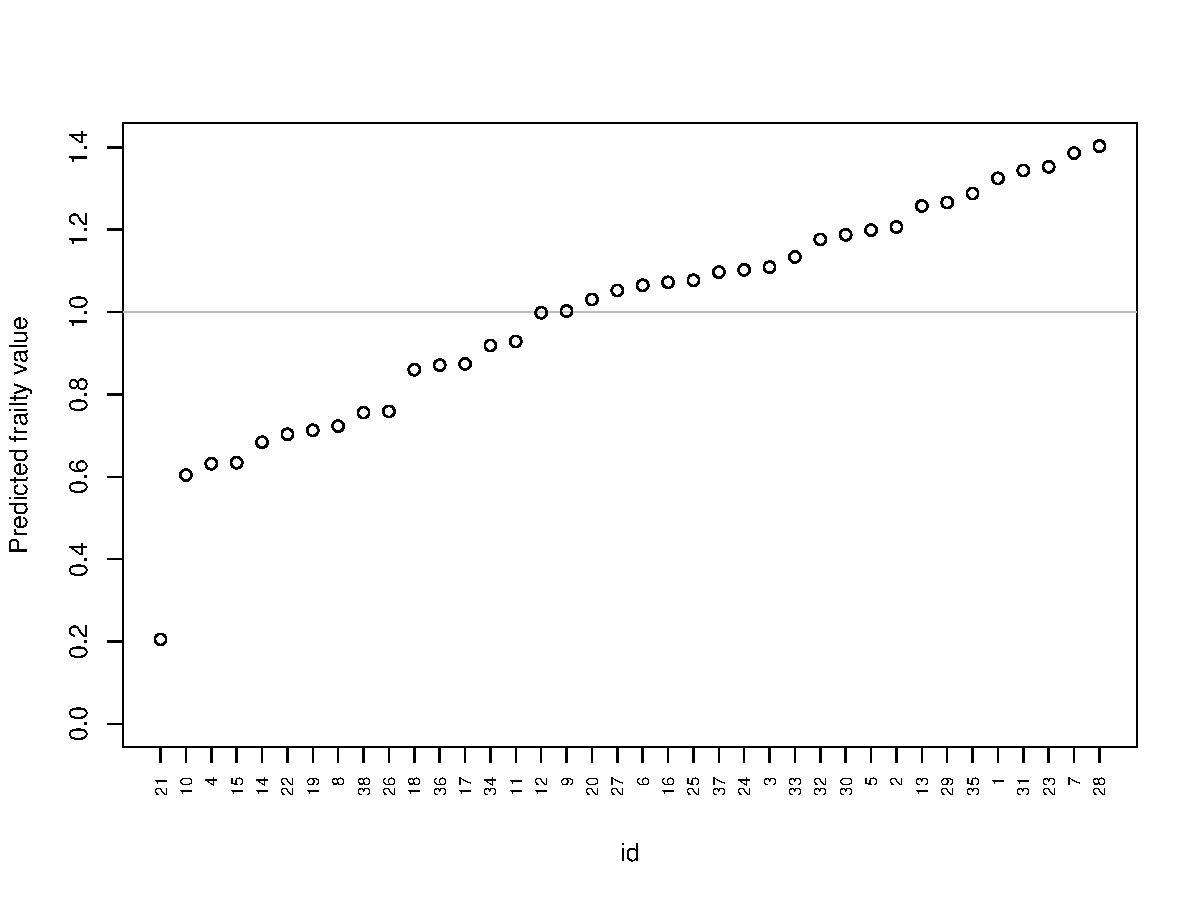
\includegraphics[width=.95\textwidth]{./graphs/prediplot.pdf}
  \caption{Prediction of frailties for the {kidney} dataset
    as given by the parametric gamma--exponential frailty model.}
  \label{fig:kidney.prediction}
\end{figure}


% % % % % % % % % % % % % % % % % % Comparison of different models % % % % % % % % % % % % % % % % % %
\paragraph{Comparison of different models.}
In some circumstances, it might be useful to easily obtain AIC and BIC values 
  for a series of candidate models. 
  This can be done using the \code{select.parfm()} function.
% The \code{select.parfm()} function is used to obtain the AIC and BIC for all candidate models.
% Even though, in clinical practice, a parametric form is assumed only in presence of strong previous information,
% \todo{ Is it clear that this is not a standard way to choose a model?}
%   this tool might help in the choice of the model.
Its use is similar to that of the \code{parfm()} function,
  but the \code{dist} and \code{frailty} values are vectors
  that contain all the alternatives to try.

\begin{CodeChunk}
\begin{CodeInput}
R> kidney.parfm <- select.parfm(Surv(time, status) ~ sex + age, 
+    cluster="id", data=kidney,
+    dist=c("exponential", "weibull", "loglogistic",
+           "lognormal", "logskewnormal"),
+    frailty=c("gamma", "ingau", "possta", "lognormal"))
R> kidney.parfm
\end{CodeInput}
\begin{CodeOutput}
 AIC:             gamma  ingau possta lognor
   exponential      674    676    682    675
   weibull          674    677    682    676
   loglogistic      685    685    686    685
   lognormal        679    679    681    679
   logskewnormal    681    681    682    681

 BIC:             gamma  ingau possta lognor
   exponential      684    685    692    685
   weibull          686    688    694    687
   loglogistic      697    697    697    696
   lognormal        691    691    692    691
   logskewnormal    695    695    696    695
\end{CodeOutput}
\end{CodeChunk}

\begin{figure}
  \centering
  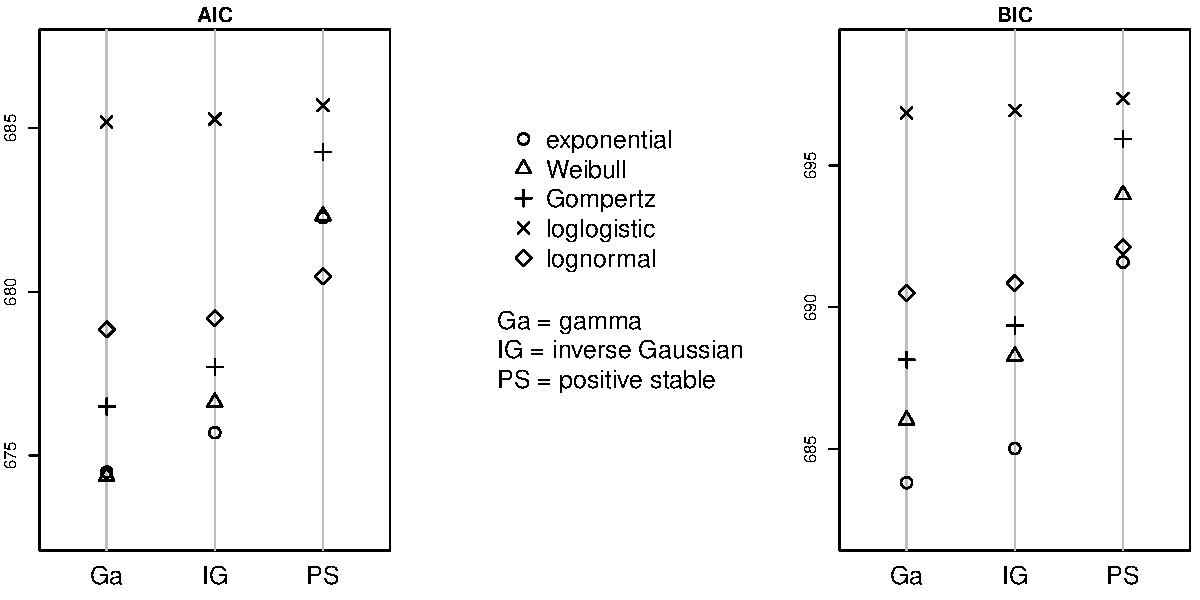
\includegraphics[width=.95\textwidth]{./graphs/plot.pdf}
  \caption{AIC and BIC values of \pkg{parfm} models for the {kidney} dataset.}
  \label{fig:kidney.parfm}
\end{figure}

The results can be plotted (Figure~\ref{fig:kidney.parfm}) via the command \code{plot(kidney.parfm)}.
In this particular example, the exponential baseline seems to be a good candidate.

As a comparison, the model with inverse Gaussian distributed frailties
  is fitted by changing the \code{frailty} argument into \code{`ingau'}.

\begin{CodeChunk}
\begin{CodeInput}
R> parfm(Surv(time, status) ~ sex + age, cluster="id", 
+        data=kidney, dist="exponential", frailty="ingau")
\end{CodeInput}
\begin{CodeOutput}
Frailty distribution: Inverse Gaussian 
Basline hazard distribution: Exponential 
Loglikelihood: -333.85 

       ESTIMATE SE    p-val    
theta   0.375   0.259          
lambda  0.022   0.013          
sex    -1.310   0.373 <.001 ***
age     0.004   0.011 0.693    
---
Signif. codes: 0 '***' 0.001 '**' 0.01 '*' 0.05 '.' 0.1 ' ' 1

Kendall's Tau: 0.125 
\end{CodeOutput}
\end{CodeChunk}

In this case, the conclusions drawn from the previous two models are essentially analogous.

Consider now the model with the positive stable frailty distribution.
In this example, it converges to a solution which is not valid ($\nu=0$)
  with the default settings.

\begin{CodeChunk}
\begin{CodeInput}
R> parfm(Surv(time, status) ~ sex + age, cluster="id", 
+        data=kidney, dist="exponential", frailty="possta")
\end{CodeInput}
\begin{CodeOutput}
Frailty distribution: Positive Stable 
Basline hazard distribution: Exponential 
Loglikelihood: -337.132 

       ESTIMATE SE p-val 
nu      0.000            
lambda  0.012            
sex    -0.885            
age     0.004            
---
Signif. codes: 0 '***' 0.001 '**' 0.01 '*' 0.05 '.' 0.1 ' ' 1

Kendall's Tau: 0 
Warning message:
In parfm(Surv(time, status) ~ sex + age, cluster = "id", data = kidney,  :
  Error in solve.default(res$hessian) : 
  Lapack routine dgesv: system is exactly singular
\end{CodeOutput}
\end{CodeChunk}

The default initial value for $\nu$ is $1/2$ in the case of positive stable frailties;
 it can be changed by means of the \code{iniFpar} option in \code{parfm()}.
Let us try with $\nu= 0.25$.

\begin{CodeChunk}
\begin{CodeInput}
R> parfm(Surv(time, status) ~ sex + age, cluster="id", 
+        data=kidney, dist="exponential", frailty="possta", 
+        iniFpar=0.25)
\end{CodeInput}
\begin{CodeOutput}
Execution time: 1.71 second(s)

Frailty distribution: Positive Stable 
Basline hazard distribution: Exponential 
Loglikelihood: -336.182 

       ESTIMATE SE    p-val    
nu      0.112   0.084          
lambda  0.014   0.008          
sex    -0.951   0.348 0.006 ** 
age     0.004   0.011 0.698    
---
Signif. codes: 0 '***' 0.001 '**' 0.01 '*' 0.05 '.' 0.1 ' ' 1

Kendall's Tau: 0.112 
\end{CodeOutput}
\end{CodeChunk}

The problem might also be fixed by changing the optimisation method (see \code{optim()}).
By default it is set to \code{`BFGS'}, 
  but it can be changed through the \code{method} option.

\begin{CodeChunk}
\begin{CodeInput}
R> parfm(Surv(time, status) ~ sex + age, cluster="id", 
+        data=kidney, dist="exponential", frailty="possta", 
+        method="Nelder-Mead")
\end{CodeInput}
\begin{CodeOutput}
Execution time: 1.51 second(s)

Frailty distribution: Positive Stable 
Basline hazard distribution: Exponential 
Loglikelihood: -336.182 

       ESTIMATE SE    p-val    
nu      0.112   0.084          
lambda  0.014   0.008          
sex    -0.951   0.348 0.006 ** 
age     0.004   0.011 0.694    
---
Signif. codes: 0 '***' 0.001 '**' 0.01 '*' 0.05 '.' 0.1 ' ' 1

Kendall's Tau: 0.112 
\end{CodeOutput}
\end{CodeChunk}

In this example the results obtained by changing the optimisation method are the same
  as those obtained by changing the initial value of $\nu$.
When convergence problems occur, using different starting values and/or different optimisation methods
  is generally sufficient to find the global maximum of the marginal likelihood function.


  
% % % Semiparametric model
Finally we provide a comparison with the semi-parametric model.
As an example, we fit the semi-parametric model with gamma frailties via the \code{coxph()} function.
\begin{CodeChunk}
\begin{CodeInput}
R> coxph(Surv(time, status) ~ sex + age +
+        frailty(id, distribution="gamma", eps=1e-11),
+        outer.max=15, data=kidney)
\end{CodeInput}
\begin{CodeOutput}
                         coef     se(coef) se2    Chisq DF   p      
sex                       -1.58323 0.4594   0.3515 11.88  1.0 0.00057
age                        0.00522 0.0119   0.0088  0.19  1.0 0.66000
frailty(id, distribution                           22.96 12.9 0.04100

     Variance of random effect= 0.408   I-likelihood = -181.6 
\end{CodeOutput}
\end{CodeChunk}

Estimates of regression parameters are quite similar to those of the exponential--gamma model,
  while the frailty variance is sensibly different,
  arguably because of the difference in how the baseline hazard is treated.

  
\section{Discussion}
  \label{sec:concl}
  To the best of our knowledge, parametric frailty models are currently especially handled in \proglang{STATA} 
  by means of the \code{streg} command.
With \pkg{parfm}, they are now readily fitted in \proglang{R}.
Further, \pkg{parfm} provides the positive stable frailty distribution 
  which is presently unavailable in \proglang{STATA}.
Actually, except for a \proglang{SAS} macro, \code{ps_frail}, 
  developed by \cite{ShuKlein99} in the semi-parametric setting, 
  we are not aware of another package that provides the positive stable frailty distribution.

% % % Parfm package features % % % 
The \pkg{parfm}~package is flexible and easy to use. 
It provides five distributions for the baseline hazard and three frailty distributions.
Parameter estimation is done by maximising the marginal log-likelihood given in Equation~\ref{eq:loglik.marg}.
The \code{optim()} function is employed, 
  and its \code{method} option is passed to \code{parfm()} (with \code{method="BFGS"} by default).
If not specified in the \code{inip} option, 
  initial values for all but the heterogeneity parameter are obtained by fitting 
  an unadjusted (i.e., without frailty) parametric proportional hazards model 
  using the \code{phreg()}~function from the \pkg{eha}~package \citep{R:eha}.
The initial heterogeneity parameter can also be specified by the user via the \code{iniFpar} option;
  otherwise it is set to $1$ when frailties follow a gamma or an inverse Gaussian distribution, 
  or to $1 \slash 2$ when they follow the positive stable distribution.

% % % No frailty estimation % % % 
Additionally, when \code{frailty="none"}, \code{parfm()} fits the unadjusted parametric proportional hazards model,
  similar to \code{survreg()} (from the \pkg{survival} package) or to \code{phreg()}.
However, \code{survreg()} returns the parameter estimates in the log-linear model 
  and \code{phreg()} uses yet another parametrisation (see the documentation).
Often, the user has then to transform back the parameters 
  and to employ the delta method in order to get estimates for the standard errors.
The \code{parfm()} function directly uses the proportional hazards representation.

% % % Problems % % % 
Nonetheless, \pkg{parfm} might reach its limits when at least one $d_i$,
  the number of events in the $i$-th cluster, $i \in \{ 1, \ldots{}, G \}$, is very large.
% 
% % PS
First, consider the positive stable distribution and observe that, 
  for a fixed value of $m \in \{1, \ldots, q-1\}$, $\Omega_{q, m}$ rapidly grows as $q$ increases; 
  see Equations~\ref{eq:PSOmegas}.
At the extreme, some of them might exceed the largest representable number in \proglang{R}.
These are then stored as \code{Inf}. 
This, in turn, prevents the marginal log-likelihood~\ref{eq:loglik.marg} to be evaluated and hence maximised.
On a side note, also the \proglang{SAS} macro \code{ps_frail} that implements the EM algorithm to fit the semi-parametric positive stable frailty model 
	has analogous difficulties when the number of events is large (or even moderate).
The following ad-hoc solution is implemented in \pkg{parfm}:
  in order to keep the polynomials $\Omega_{q, m}$'s reasonably small, 
  they are divided by some factor $10^{K}$ which does not change the marginal log-likelihood
	except for an additive constant (equal to $s \times K \times \log ( 10 )$).
The value of $K$ is specified via the \code{correct}~option (default is \code{correct=0}, i.e., no correction)
	and \code{parfm()} returns the re-adjusted log-likelihood value.
That solution serves the purpose for moderately large values of $d_{i}$ 
  (say up to about $200$ events per cluster according to our experience, 
  but it depends on the data, on the other parameters,
  and on the hardware characteristics).
%   
% % IG
With the inverse Gaussian distribution, 
  the Bessel function $K_{q - 1 \slash 2} ( z )$ in Equation~\ref{eqn:ingau} raises the same problem.
Indeed, it explodes when $z$ is small relative to $q$; see Figure~\ref{fig:bessel}.
Currently, that distribution should, therefore, preferably be avoided when there are very 
  large values of $d_{i}$ (say above $200$ events per cluster according to our experience,
  but, again, it depends on the data, on the other parameters and on the hardware characteristics).
Moreover, $K_{q - 1 \slash 2} ( z )$ rapidly goes to zero as $z$ increases. 
So, in case of very small apparent heterogeneity, $\theta \rightarrow 0$ which implies $z \rightarrow \infty$, 
	$K_{q - 1 \slash 2} ( z )$ might be stored as $0$ in \proglang{R} and hence $\log( K_{q - 1 \slash 2} ( z ) )$ 
	cannot be computed.
However, 
  as this problem occurs in the case of very small heterogeneity,
  this would rather suggest to fit the model with \code{frailty="none"}.	
  % 
  \begin{figure}[htbp]
  \centering
  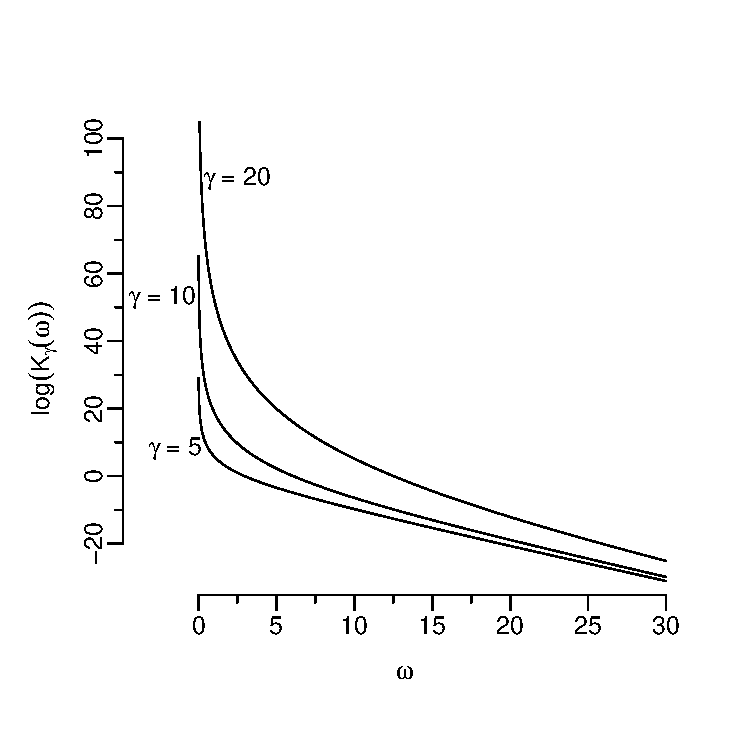
\includegraphics[width=.6\textwidth]{./graphs/bessel.pdf}
  \caption{The logarithm of the Bessel function, $\log ( K_{\gamma} ( \omega ) )$, versus $\omega$ for different values of $\gamma$.} 
  \label{fig:bessel}
  \end{figure}
  % 
% 
% % gamma
When frailties are gamma distributed,
  which is by far the most popular assumption in common practice, 
  the quantities involved in Equation~\ref{eqn:gamma} do not raise any worry.
In practice, even when dealing with datasets with huge numbers of events per cluster,
  there is no real risk of exceeding the range of floating-point numbers.


% \clearpage
% Bibliography
% \bibliographystyle{jss}
\bibliography{tex/lib}

\clearpage
\appendix
\section{Proofs}
\subsection{Derivatives of the Laplace transform of the inverse Gaussian frailty distribution} 
  \label{app:derLTIG}
  On the one hand, for any frailty distribution $f ( u_{i} ; \xi )$, 
  the $\alpha$-th moment of $U$ ($\alpha \in \mathbb N$),
  conditional on the data from the $i$-th cluster and on the parameters,
  can be written in the form 
\begin{equation} \label{eq:condEfrailty}
  \E(U^{\alpha} \mid \bm z_i, \bm \tau_i; \bm\psi, \bm\beta, \xi) = \frac{
    \E \left( U^{d_i + \alpha} \exp\left( 
      -U H_{i\cdot,c}(\bm y_i)
%       \sum_{j = 1}^{n_i} H_0(y_{ij}) \exp(\bm x^\top_{ij} \bm\beta) 
      \right)\right)
  }{
    \E \left( U^{d_i} \exp\left(
      -U H_{i\cdot,c}(\bm y_i)
%       \sum_{j = 1}^{n_i} H_0(y_{ij}) \exp(\bm x^\top_{ij} \bm\beta ) 
    \right) \right)}
  \ccom
\end{equation}
with
$H_{i\cdot,c}(\bm y_i) = \sum_{j=1}^{n_i} H_0 ( y_{ij} ) \exp ( \bm x^\top_{ij} \bm\beta )$.

This is a generalisation of a result found by \cite{WangEtal95} which follows from Bayes's formula applied to $f ( u_{i} \mid \bm{z}_{i}, \bm{\tau}_i ; \bm{\psi}, \bm{\beta}, \xi )$ in
\[
 \E \left( U^\alpha \mid \bm z_i, \bm \tau_i ; \bm\psi, \bm\beta, \xi \right) 
  = \int_0^\infty u_i^\alpha f \left( u_i \mid \bm z_i, \bm \tau_i ; \bm\psi, \bm\beta, \xi \right) \mathrm d u_i 
\]
(see Appendix~\ref{app:condEfrailty} for more details).
%   
Now, since the expected values in the right-hand side of Equation~\ref{eq:condEfrailty}
  can be written in terms of derivatives of the Laplace transform
\[
  \E \left( U^q \exp(-sU) \right) = (-1)^q \mathcal L^{(q)}(s), \qquad q, s \geq 0,
\]
we have that
\begin{equation} \label{eq:dLTrecurs}
  \mathcal{L}^{( d_{i} + \alpha )} \left( 
    H_{i\cdot,c}(\bm y_i)
%     \sum_{j = 1}^{n_{i}} H_{0} ( y_{ij} ) \exp ( \bm{x}^\top_{ij} \bm{\beta} ) 
    \right) =
    ( - 1 )^{\alpha} \E ( U^{\alpha} \mid \bm{z}_{i}, \bm{\tau}_i; \bm{\psi}, \bm{\beta}, \xi ) 
    \ \mathcal{L}^{( d_{i} )} \left( 
    H_{i\cdot,c}(\bm y_i)
%     \sum_{j = 1}^{n_{i}} H_{0} ( y_{ij} ) \exp ( \bm{x}^\top_{ij} \bm{\beta} ) 
    \right).
\end{equation}

On the other hand, if $U \sim \textrm{IG}^\star (\theta)$, 
  then it is easy to show (Appendix~\ref{app:condIG})
  that the conditional distribution of $U$ given the data and the parameters is a 
  generalised inverse Gaussian distribution:
  \[
   U \mid \bm{z}_{i}, \bm \tau_i; \bm{\psi}, \bm{\beta}, \theta
    \sim \mathrm{GIG} (\gamma_{_{\mathrm{GIG}}}, \delta_{_{\mathrm{GIG}}}, \theta_{_{\mathrm{GIG}}} )
  \]
  with
  \begin{align} \label{eq:GIGpar1}
    \gamma_{_{\textrm{GIG}}} &= d_i - \frac12\ccom \\
    \theta_{_{\textrm{GIG}}} &= \frac1{2 \theta} + H_{i\cdot,c}(\bm y_i), \\
%       \sum_{j = 1}^{n_{i}} H_{0} ( y_{ij} ) \exp ( \bm{x}^\top_{ij} \bm{\beta} ), \\
    \delta_{_{\textrm{GIG}}} &= \frac1{\sqrt{2 \theta}}\cdot
    \label{eq:GIGpar3}
  \end{align}

Hence \cite[Section A.3.6]{Hougaard00}
\begin{equation} \label{eq:condEfIG}
  \E ( U^{\alpha} \mid \bm{z}_{i}, \bm{\tau}_i; \bm{\psi}, \bm{\beta}, \xi ) = 
    \left( \frac{\theta^{1 \slash 2}_{_{\textrm{GIG}}}}{\delta_{_{\textrm{GIG}}}} \right)^{- \alpha}
    \frac{K_{\gamma_{_{\textrm{GIG}}} + \alpha} ( 2 \delta_{_{\textrm{GIG}}} \theta^{1 \slash 2 }_{_{\textrm{GIG}}} )}
          {K_{\gamma_{_{\textrm{GIG}}}} ( 2 \delta_{_{\textrm{GIG}}} \theta^{1 \slash 2 }_{_{\textrm{GIG}}} )}
    \cdot
\end{equation}

Combining (\ref{eq:dLTrecurs}) and (\ref{eq:condEfIG}), Equation~\ref{eq:invGauss} is deduced.
\qed

  
\clearpage
\subsection{Conditional expectation of frailty terms}
  \label{app:condEfrailty}
  For ease of notation, let $H_{i\cdot,c}(\bm y_i)$ denote 
  $\sum_{j=1}^{n_i} H_0 ( y_{ij} ) \exp ( \bm x^\top_{ij} \bm\beta )$.

For any frailty distribution $f(u_i; \xi)$ and for any $\alpha \in \mathbb N$, we have
  
\begin{align*}
\E \left( U^\alpha \mid \bm z_i, \bm \tau_i ; \bm\psi, \bm\beta, \xi \right) 
  &= \int_0^\infty u_i^\alpha f \left( u_i \mid \bm z_i, \bm \tau_i ; \bm\psi, \bm\beta, \xi \right) \mathrm d u_i \\
  &=  \int_0^\infty u_i^\alpha \frac{L_{\mathrm{cond}} \left( \bm\psi, \bm\beta \mid \bm \tau_i, u_i; \bm z_i \right) f \left( u_i \mid \bm \tau_i ; \xi \right) }
      {L_{\mathrm{marg}} \left( \bm\psi, \bm\beta, \xi \mid \bm \tau_i ; \bm z_i \right)} \mathrm d u_i,
\end{align*}

with

\begin{eqnarray*}
L_{\mathrm{cond}} \left( \bm\psi, \bm\beta \mid \bm \tau_i, u_i; \bm z_i \right) & = & \left[ \prod_{j=1}^{n_i} \left( h_0 ( y_{ij} ) u_i \exp ( \bm x^\top_{ij} \bm\beta ) \right)^{\delta_{ij}} \right]  \exp \left( - u_i  H_{i\cdot,c}(\bm y_i) \right) \exp \left( u_i  H_{i\cdot,c}(\bm \tau_i)  \right), \\
f \left( u_i \mid \bm \tau_i ; \xi \right) & = & \frac{\exp \left( -u_i  H_{i\cdot,c}(\bm \tau_i)  \right) f(u_{i}; \xi)}{\mathcal{L} \left(H_{i\cdot,c}(\bm \tau_i)\right)}\ccom \\
L_{\mathrm{marg}} \left( \bm\psi, \bm\beta, \xi \mid \tau_i ; \bm z_i \right) & = & \int_{0}^{\infty} L_{\mathrm{cond}} \left( \bm\psi, \bm\beta \mid \bm \tau_i, u_i; \bm z_i \right) f \left( u_i \mid \bm \tau_i ; \xi \right) \mathrm du_{i}.
\end{eqnarray*}

Thus,

\begin{align*}
\E \left( U^\alpha \mid \bm z_i, \bm \tau_i ; \bm\psi, \bm\beta, \xi \right)
 &= \frac{\displaystyle \int_0^\infty u_i^{d_i + \alpha} \exp \left( - u_i  H_{i\cdot,c}(\bm y_i) \right) f(u_i ; \xi) \mathrm d u_i}
        {\displaystyle \int_0^\infty u_i^{d_i} \exp \left( - u_i  H_{i\cdot,c}(\bm y_i) \right) f(u_i ; \xi) \mathrm d u_i} \\
   &= \frac{\displaystyle E \left[ U^{d_i + \alpha} \exp \left( -U  H_{i\cdot,c}(\bm y_i) \right) \right]}{\displaystyle E \left[ U^{d_i} \exp \left( -U  H_{i\cdot,c}(\bm y_i) \right) \right]}\cdot
\end{align*}
\qed

\clearpage
\subsection{Conditional distribution of inverse Gaussian frailty} 
  \label{app:condIG}
  Let $U \sim \textrm{IG}^{\star} ( \theta)$, then the distribution of 
  $U \mid \bm{z}_{i}, \bm \tau_i; \bm{\psi}, \bm{\beta}, \theta$ is
\begin{eqnarray*}
f ( u_i \mid \bm{z}_{i}, \bm{\tau}_i; \bm{\psi}, \bm{\beta}, \theta ) 
  & = & \frac{
    L_{\textrm{cond}} \left( \bm{\psi}, \bm{\beta} \mid \bm{\tau}_{i}, u_{i}; \bm{z}_i \right) f ( u_{i} \mid \bm{\tau}_{i}; \theta )
  }{
    L_{\textrm{marg}} \left( \bm{\psi}, \bm{\beta}, \theta \mid \bm{\tau}_{i}; \bm{z}_i \right)
  } \\
  &\propto & L_{\textrm{cond}} \left( \bm{\psi}, \bm{\beta} \mid \bm{\tau}_{i}, u_{i}; \bm{z}_i \right) f ( u_{i} \mid \bm{\tau}_{i}; \theta ) \\
  & \propto & \displaystyle \left[ 
      \prod_{j=1}^{n_{i}} \left( h_{0} ( y_{ij} ) u_i \exp ( \bm{x}^\top_{ij} \bm{\beta} ) \right)^{\delta_{ij}} 
    \right] 
    \exp \left( - \sum_{j=1}^{n_{i}} H_{0} ( y_{ij} ) u_i \exp ( \bm{x}^\top_{ij} \bm{\beta} ) \right) \\
    && \qquad \times \sqrt{\frac{1}{2 \pi \theta}} 
    u_i^{-\tfrac32} 
    \exp \left( -\frac{1}{2 \theta u_{i}} ( u_i - 1 )^{2} \right)   \\
  &\propto& u_i^{d_i - \tfrac32} \exp \left( - u_i 
    \left[\sum_{j=1}^{n_{i}} H_{0} ( y_{ij} ) \exp ( \bm{x}^\top_{ij} \bm{\beta} ) \right] - 
          \frac{1}{2 \theta} u_i - \frac{1}{2 \theta} \frac{1}{u_{i}} \right) \\
  & = & u_{i}^{d_i - \tfrac32} \exp \left( - \left( \frac{1}{2 \theta} + \sum_{j=1}^{n_{i}} H_{0} ( y_{ij} ) \exp ( \bm{x}^\top_{ij} \bm{\beta} ) \right) u_i - 
          \frac{1}{2 \theta} \frac{1}{u_{i}} \right),
\end{eqnarray*}
which is proportional to the density of a generalised inverse Gaussian distribution \cite[Section~A.3.6]{Hougaard00}
with parameters given by Equations~\ref{eq:GIGpar1}--\ref{eq:GIGpar3}.
\qed

\end{document}
